\section[Problem 5]{Recall our notation for the dihedral group $D_n, n \geq 1$.
    We have $x,y\in D_n$ such that the orders $o(x) = n, o(y)=2, yx = x^{-1}y$ and $D_n = <x,y>$.}
    \subsection[(i)]{Write down the element $x^2yx^{-1}y^{-1}x^3y^3$ of $D_n$
        in the form $x^iy^i$, for integers $i,j \geq 0$.}

        We have $x^n = 1, y^2 = 1, yx = x^{-1}y$.
        Now, 
        \begin{align*}
            yx &= x^{-1}y \\
            y &= x^{-1}y x^{-1} \\
            xy &= y x^{-1} \\
            % 
            \to & x^2yx^{-1}y^{-1}x^3y^3 \\
            = & x^2yx^{-1}y^{-1}x^3y \\
            = & x (y x^{-1}) x^{-1}y^{-1}x^2 (y x^{-1}) \\
            = & x y x^{-2}y^{-1}x^2 y x^{-1} \\
            = & y x^{-3}y^{-1} y x^{-3} \\
            = & y x^{-3} x^{-3} \\
            = & y x^{-6} \\
            = & x^6 y \\
            \to & i = 6, j = 1
        \end{align*}


    \subsection[(ii)]{Let $G$ be a group. Show that for all $a\in G$, if the subset $\set{1,a}$
        is a normal subgroup of $G$ then $a$ is in the center of $G$.
        Prove that $N = \set{1, x^5}$ is a normal subgroup of $D_{10}$.}
        
        Suppose $a\in G$ such that $\set{1,a}$ is a normal subgroup of $G$.
        % So $\lall g \in G, gag^{-1} \in \set{1,a}$.

        Let $x \in G$.
        Since $\set{1,a}$ is a normal subgroup of $G, xax^{-1} \in \set{1,a}$.
        If $xax^{-1} = a$, then $xa = ax$, we're done.
        If $xax^{-1} = 1$, then $a = 1$, so $xa = ax$.
        \qed

        % We need to prove $N = \set{1,x^5}$ is a normal subgroup of $D_{10}$.

        We have $x,y \in D_{10}, x^{10} = 1, y^2 = 1, yx = x^{-1}y$.

        Let $h \in N = \set{1,x^5}$. $h = 1$ is the trivial case, so assume $h = x^5$.

        Now, $x x^5 x^{-1} = x^5 \in N$, and $y x^5 y^{-1} = x^{-5} y y^{-1} = x^{-5} = x^5 \in N$.
        And any combination of $x$ and $y$ would yield the same result.
        Therefore $N$ is a normal subgroup of $D_{10}$.
        \qed
        
        

    \subsection[(iii)]{Compute the left cosets of $N$ in $D_{10}$ and show that the quotient group
        $\frac{D_{10}}{N}$ is isomorphic to $D_5$.}

        \(
            \set{
                \set{1, x^5},
                \set{x, x^6},
                \set{x^2, x^7},
                \set{x^3, x^8},
                \set{x^4, x^9},
                \set{y, yx^5},
                \set{yx, yx^6},
                \set{yx^2, yx^7},
                \set{yx^3, yx^8},
                \set{yx^4, yx^9}
            }
        \).

        We find a bijective group homomorphism from $D_{10}/N$ to $D_5$.

        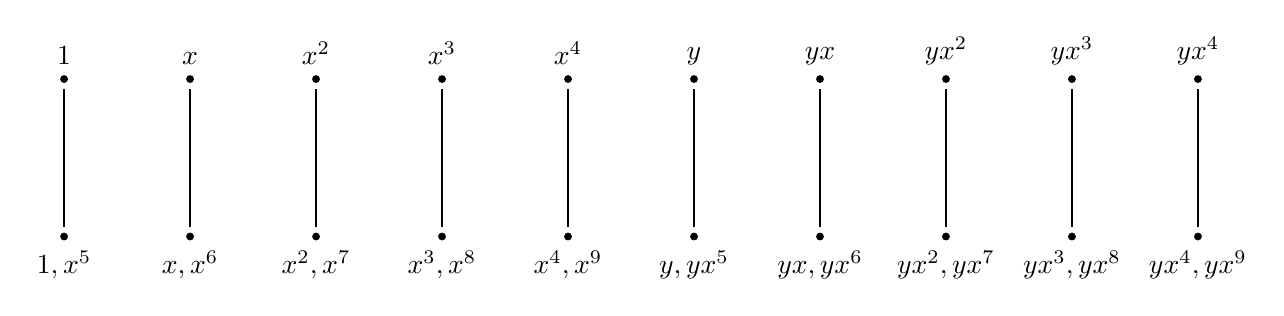
\begin{tikzpicture}[
            ele/.style={fill=black,circle,minimum width=.8pt,inner sep=1pt}
        ]
            \node[ele,label=above:$1$] (b1) at (0,2) {};
            \node[ele,label=above:$x$] (b2) at (1.6,2) {};    
            \node[ele,label=above:$x^2$] (b3) at (3.2,2) {};
            \node[ele,label=above:$x^3$] (b4) at (4.8,2) {};
            \node[ele,label=above:$x^4$] (b5) at (6.4,2) {};
            \node[ele,label=above:$y$] (b6) at (8,2) {};
            \node[ele,label=above:$yx$] (b7) at (9.6,2) {};    
            \node[ele,label=above:$yx^2$] (b8) at (11.2,2) {};
            \node[ele,label=above:$yx^3$] (b9) at (12.8,2) {};
            \node[ele,label=above:$yx^4$] (b10) at (14.4,2) {}; 

            \node[ele,label=below:$\set{1, x^5}$] (a1) at (0,0) {};
            \node[ele,label=below:$\set{x, x^6}$] (a2) at (1.6,0) {};    
            \node[ele,label=below:$\set{x^2, x^7}$] (a3) at (3.2,0) {};
            \node[ele,label=below:$\set{x^3, x^8}$] (a4) at (4.8,0) {};
            \node[ele,label=below:$\set{x^4, x^9}$] (a5) at (6.4,0) {};
            \node[ele,label=below:$\set{y, yx^5}$] (a6) at (8,0) {};
            \node[ele,label=below:$\set{yx, yx^6}$] (a7) at (9.6,0) {};    
            \node[ele,label=below:$\set{yx^2, yx^7}$] (a8) at (11.2,0) {};
            \node[ele,label=below:$\set{yx^3, yx^8}$] (a9) at (12.8,0) {};
            \node[ele,label=below:$\set{yx^4, yx^9}$] (a10) at (14.4,0) {}; 

            \draw[thick,shorten <=2pt,shorten >=2pt] (a1) -- (b1);
            \draw[thick,shorten <=2pt,shorten >=2pt] (a2) -- (b2);
            \draw[thick,shorten <=2pt,shorten >=2pt] (a3) -- (b3);
            \draw[thick,shorten <=2pt,shorten >=2pt] (a4) -- (b4);
            \draw[thick,shorten <=2pt,shorten >=2pt] (a5) -- (b5);
            \draw[thick,shorten <=2pt,shorten >=2pt] (a6) -- (b6);
            \draw[thick,shorten <=2pt,shorten >=2pt] (a7) -- (b7);
            \draw[thick,shorten <=2pt,shorten >=2pt] (a8) -- (b8);
            \draw[thick,shorten <=2pt,shorten >=2pt] (a9) -- (b9);
            \draw[thick,shorten <=2pt,shorten >=2pt] (a10) -- (b10);
        \end{tikzpicture}
        \qed